%%%%%%%%%%%%%%%%%%%%%%%%%%%%%%%%%%%%%%%%%%%%%%%%%%%%%%%%%%%%%%%%%%%%%%%%%%%

\documentclass{standalone}

\usepackage{mathptmx}
\usepackage{tikz}
\usetikzlibrary{external}
\tikzexternalize{circle-square}

%% We default to Times.
\renewcommand{\rmdefault}{ptm}
\renewcommand{\ttdefault}{pcr}
%% Enable Times/Palatino main text font.
\normalfont\selectfont

\newcommand{\comma}{,\,}
\newcommand{\tuple}[2]{({#1}\comma {#2})}

%% A general circle.
\newcommand{\myCircle}{%%
  %% Draw the circle.
  \draw[lineStyle] (centre) circle[radius=\radius];
  %% Label the centre of the circle.
  \node[nodeStyle] at (centre) {};
  \node at (centre) [below] {$\tuple{0}{0}$};
}

%% A square that is inscribed inside a circle.
\newcommand{\mySquare}{%%
  %% Draw the inscribed square.
  \draw[lineStyle] (\xlow+\dx,\ylow) -- ++(-\dx,\dy) -- ++(-\dx,-\dy)
  -- ++(\dx,-\dy) -- ++(\dx,\dy) -- cycle;
  %% Label two points where the circle meet the square.
  %% Point A.
  \node[nodeStyle] at (A) {};
  \node at (A) [right] {$A = \tuple{1}{0}$};
  %% Point B.
  \node[nodeStyle] at (B) {};
  \node at (B) [above] {$B = \tuple{0}{1}$};
}

%% Approximating pi with an inscribed square.

\begin{document}

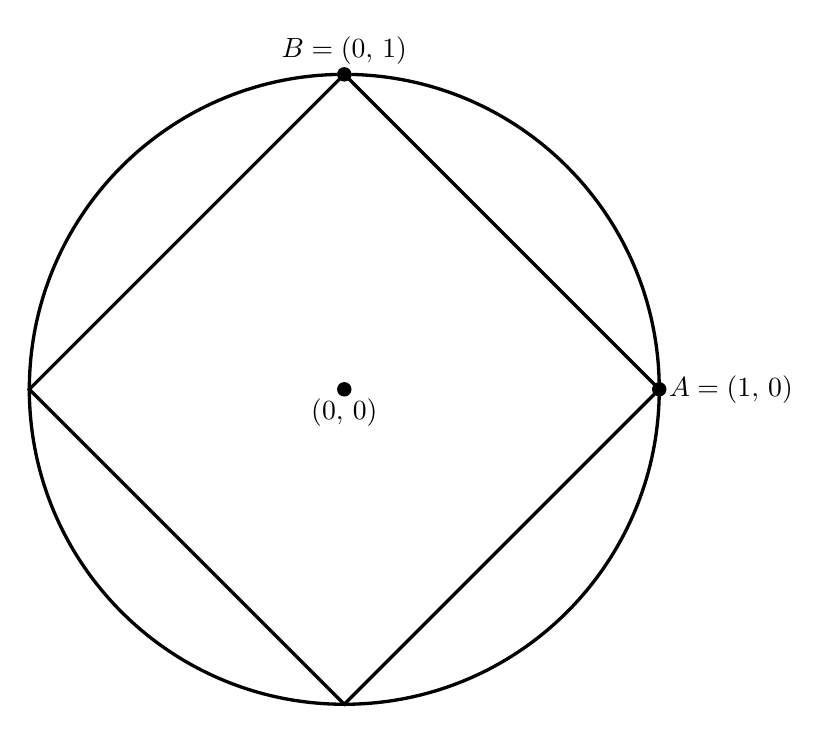
\begin{tikzpicture}[%%
  lineStyle/.style={-,very thick},%%
  nodeStyle/.style={draw,inner sep=1.7pt,circle,fill=black,black}
]
%%
%%
\pgfmathsetmacro{\radius}{4}
\pgfmathsetmacro{\dx}{\radius}
\pgfmathsetmacro{\dy}{\dx}
\pgfmathsetmacro{\xlow}{0}
\pgfmathsetmacro{\ylow}{0}
\coordinate (A) at (\xlow+\dx,\ylow);
\coordinate (B) at (\xlow,\ylow+\dy);
\coordinate (centre) at (\xlow,\ylow);
%%
%% Draw a circle with an inscribed square.
\myCircle
\mySquare

\end{tikzpicture}

\end{document}
